%Max 1500w or 4 pages
%Deadline 17:00 on Tuesday 09-02-2016

\section{Introduction}

The project aims to create a micro-modelled road traffic simulation engine enabling inspection of various effects of changing key rules within the model. For team members, this project is centered around teamwork and also, as a less prominent addition, the learning and application of software engineering skills within a group setting.

\section{Project Description} %~60% of the report
%Describe your team’s aims for the projects. Outline what aims your team have set for the project and your strategy for achieving those aims. A rough timetable may be appropriate and you may wish to break your aims into levels (e.g. mandatory / optional or we will first work on level 1 aims before moving to level 2 aims) to allow for unexpected issues that may arise. You must also describe how your initial progress developing your piece of software has gone and where you currently are relative to your aims.

\subsection{Simulation Model}
The project started with a research phase to determine the general approaches to micro and macro models in order to decide which one the team would use for the simulation. After a vote the micro model was unanimously chosen for its precise granular control over the agents down to the individual ones within the simulation.

\vspace{3mm}

As the micro-model implementation focuses on individual representation of cars as physical objects and individual tuning of their parameters the starting point chosen is based on the Nagel–Schreckenberg model. The roads in this model are represented as cellular automata\cite{Schreckenberg}. In this, each cell can either be occupied by an object or be empty. Cars can have different properties such as acceleration, speed, direction and can move to other free neighbouring cells. The model can be expanded through the use of graphs to connect roads.

\vspace{3mm}

In the early stages streets will be arranged to model simple road networks and, in later ones, more realistic ones.
Rules in the simulation will include driving rules such as crossings, lane changes, etc.., and laws of physics. That can be further expanded to include weather factors and engine emissions for example.

\vspace{3mm}

The simulation system will be used to gather relevant data on the reaction of the model to changing rules for analysis. This will include road network throughput and congestion effects.

\subsubsection{Architecture}

A brainstorming session hewed a rough architectural outlay of the product. It breaks down into three main artefacts:
\vspace{1mm}
\begin{itemize}
	\item the GUI,
	\item the simulation engine and
	\item a log library module
\end{itemize}
\vspace{1mm}
The simulation engine will be broken up into smaller pieces as it is not only the centrepiece of the project but also the biggest part (see Figure~\ref{fig:arch_overview}).

\begin{figure}[h!]
	\vspace{1.5em}
  	\caption{Rough architecture overview}
  	\label{fig:arch_overview}
  	\centering
	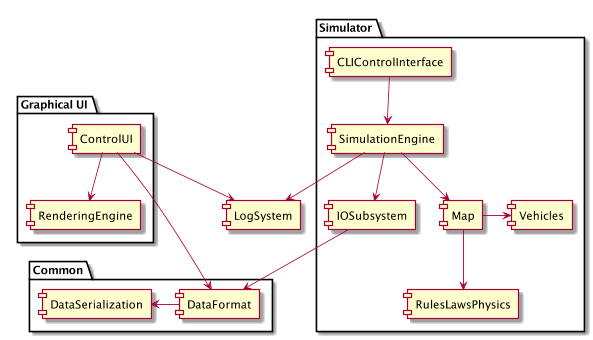
\includegraphics[width=0.5\textwidth]{figs/arch_diagram.png}
  	\vspace{1.5em}
\end{figure}

\subsection{Development}

Once a rough architecture and the tooling is set-up the plan is to start developing modules as early as possible to get a basic system working before reaching the 2\textsuperscript{nd} milestone so as to have a buffer in the event of unforeseen setbacks.

\vspace{3mm}

Java was chosen as the development language as all members of the team have, at the very least, some familiarity with it. It also is cross-platform, has GUI capabilities and has a slew of libraries and tools available for it.
	
\subsection{Preliminary Timetable \& Current project status}
 
The timetable is broken into 4 major milestones and each of those encompass a set of goals to be completed by the date (see Table~\ref{tab:milstones}). 
\vspace{3mm}

\begin{table}[h]
	\vspace{1.5em}
	\caption{Preliminary Milestones descriptions and current statuses}
	\label{tab:milstones}
	\centering
	\resizebox{\linewidth}{!}{%
\begin{tabular}{lc}
\rowcolor[HTML]{656565} 
{\color[HTML]{FFFFFF} \textbf{Milestone timetable}} & {\color[HTML]{FFFFFF} \textbf{Status}} 					\\ \hline
\multicolumn{2}{l}{\textbf{9th Feb - Milestone I: Preliminary report submission}}       						\\ \hline
Team structure ready           																					& \checkmark \\
Team process setup (communication, teamwork, knowledge sharing, visibility)         							& \checkmark \\
Graple deployment harness																						& \checkmark \\
Basic log system																								& \checkmark \\
Rough architecture outlined, some basics set for modelling		                    							& \checkmark \\ \hline
\multicolumn{2}{l}{\textbf{1st Mar - Milestone II: Basic Functionalities implemented and working}}   			\\ \hline
Basic modelling ready: simple roads with different physical object properties									& \\
Basic tooling support: setting up testbed parameters, map, parameters of active objects 			       		& \\
Full multi-output (terminal, txt file and csv file) functionalities in Log system completed						& \\
Basic measurements ready: log output, throughput measurements, simulation saving								& \\ 
Basic GUI ready: display animations either from live simulation or saved as a file 								& \\ \hline
\multicolumn{2}{l}{\textbf{25th Mar - Milestone III: Possible advanced functionalities implemented and working}}\\ \hline
Optional: Larger size of the model: graph with many connections                									& \\
Optional: Loading map data from actual OpenStreetMap sources (filtering highways, counting lanes, etc...) 		& \\
Optional: Attempting in-model traffic lights and model parameters optimization with different algorithms        & \\ \hline
\multicolumn{2}{l}{\textbf{31st Mar - Milestone IV: Final report submission}}		\\ \hline
Code prepared and ensured for correctness and visibility 														& \\
Report ready and submitted. 																					& \\
Presentation ready \& rehearsed 																				& \\ \hline
\end{tabular}}
	\vspace{1.5em}
\end{table}

As the table describes, the team has already completed all the set-ups of processes to facilitate development and communication, and has also started coding the log module necessary to facilitate hunting down any issues in the code when run when they arise. Essentially, the 1\textsuperscript{st} milestone's tasks have been completed ahead of time.

\section{Project Organisation} %~40% of the report
Describe how you will work together as a team. You should set out the roles you expect team members to play and what
processes and tools you will use to collaborate together as a team. You should also explain the process you expect to
use for handling peer assessment as well as the mechanisms you have agreed upon for handling any conflicts within the
team that may arise.

\begin{itemize}
	\item Teamwork
	\begin{itemize}
		\item Distribution of tasks
    	\item Conflict resolution
    	\item Efforts planned from each member
    	\item Meetings (could tie in the tools in this section?)
        \begin{enumerate}
            \item Organisation of matters to discuss
            \item Organisation of meeting time
        \end{enumerate}
        \item peer assesment (marks)

        \item Process
        \begin{itemize}
            \item Kanban-like process with board and no strict iterations defined
            \item Minimum viable product set out rather early (half-time) so should have features to add on later
            \item Git: for now master-only, will switch to features branches as everyone is comfy with git
            \item Test: obligatory automated unit-testing for components and features
            \item Peer review: post-commit review of features (peer). At least 1 person should have looked at code after commit.
        \end{itemize}
	\end{itemize}

	\item Tools
	\begin{itemize}
		\item Trello
		\item HipChat (inc. Git commit \& trello plugin)
	    \item JetBrain's IntelliJ Idea IDE for everyone
	    \item PlantUML for UML diagrams?
	\end{itemize}

\end{itemize}



